%%%%%%%%%%%%%%%%%%%%%%%%%%%%%%%%%%%%%%%%%
% MUW Poster
% LaTeX Template
% Version 1.0 (31/08/2016)
% (Based on Version 1.0 (31/08/2015) of the Jacobs Portrait Poster
%
% License:
% CC BY-NC-SA 3.0 (http://creativecommons.org/licenses/by-nc-sa/3.0/)
%
% Created by:
% Nicolas Ballarini, CeMSIIS, Medical University of Vienna
% nicoballarini@gmail.com
% http://statistics.msi.meduniwien.ac.at/
%%%%%%%%%%%%%%%%%%%%%%%%%%%%%%%%%%%%%%%%%


\def\footer#1{\def\insertfooter{#1}}
%--------------------------------------------------------------------------------------
%	PACKAGES AND OTHER DOCUMENT CONFIGURATIONS
%--------------------------------------------------------------------------------------

\documentclass[final]{beamer}

\usepackage[scale=1.150]{beamerposter} % Use the beamerposter package
\usetheme{MUWposter} % Use the MUWposter theme supplied with this template
\usepackage{color, colortbl}
\definecolor{gray}{gray}{0.9}
\usepackage{multicol}
\usepackage{array}
\newcolumntype{L}{>{\arraybackslash}m{22cm}}
\newcolumntype{S}{>{\arraybackslash}m{5cm}}
\usepackage{pgf}  
\usepackage{mathtools}
\usepackage{amsmath, amsthm, amssymb, amsfonts}
\usepackage{exscale}
\usepackage{xcolor}
\usepackage{ushort}
\usepackage{setspace}
\usepackage[square,numbers]{natbib}
\usepackage{url}
\bibliographystyle{apalike}
\renewcommand{\vec}[1]{\ushort{#1}}
\renewcommand{\vec}[1]{\mathbf{#1}}
\definecolor{greenMUW}{RGB}{29,150,55}
\definecolor{blueMUW}{RGB}{17,29,79}
\definecolor{skinMUW}{RGB}{254,228,217}
\definecolor{hellblauMUW}{RGB}{95,180,229}
\usepackage{subfig}

%-----------------------------------------------
%  START Set the colors
%  Uncomment to apply colors you want to use.
%-----------------------------------------------
\colorlet{themecolor}{greenMUW}
\usebackgroundtemplate{
\includegraphics{images/UCD_back.pdf}}

%-----------------------------------------------
%  END Set the colors
%-----------------------------------------------


%-----------------------------------------------
%  START Set the width of the columns
%-----------------------------------------------
\setlength{\paperwidth}{33.1in} % A0 width: 46.8in
\setlength{\paperheight}{46.8in} % A0 height: 33.1in
\newlength{\sepmargin}
\newlength{\sepwid}
\newlength{\onecolwid}
\newlength{\twocolwid}
\newlength{\threecolwid}

% The following measures are used for 2 columns
\setlength{\sepmargin}{0.055\paperwidth} % Separation width (white space) between columns
\setlength{\sepwid}{0.03\paperwidth} % Separation width (white space) between columns
\setlength{\onecolwid}{0.43\paperwidth} % Width of one column
\setlength{\twocolwid}{0.9\paperwidth} % Width of two columns

%-----------------------------------------------------------
% The following measures are used for 3 columns
%\setlength{\sepmargin}{0.06\paperwidth} % Separation width (white space) between columns
%\setlength{\sepwid}{0.02\paperwidth} % Separation width (white space) between columns
%\setlength{\onecolwid}{0.28\paperwidth} % Width of one column
%\setlength{\twocolwid}{0.58\paperwidth} % Width of two columns
%\setlength{\threecolwid}{0.88\paperwidth} % Width of three columns
%\setlength{\columnsep}{30pt}

%-----------------------------------------------
%  END Set the width of the columns
%-----------------------------------------------


%--------------------------------------------------------------------------------------
%	TITLE SECTION 
%--------------------------------------------------------------------------------------
\setbeamertemplate{title}[left]
\setbeamertemplate{frametitle}[default][left]

\title{\huge{The Relationship Between Corporate Governance and \\~\\ Company Performance}} % Poster title

\author{Conor Reid - {\large MSc Business Analytics}} % Author(s)

\institute{\large Supervisors - Dr. James McDermott and Dr. Miguel Nicolau} % Institution(s)
%--------------------------------------------------------------------------------------

\begin{document}
  \addtobeamertemplate{block end}{}{\vspace*{1ex}} % White space under blocks
  \addtobeamertemplate{block alerted end}{}{\vspace*{0ex}} % White space under highlighted (alert) blocks
  \setlength{\belowcaptionskip}{2ex} % White space under figures
  \setlength\belowdisplayshortskip{1ex} % White space under equations
  
\begin{frame}[t] % The whole poster is enclosed in one beamer frame
\begin{columns}[t] % The whole poster consists of two major columns
\begin{column}{\sepmargin}\end{column}


%--------------------------------------------------------------------------------------------------------------------------------------------------------------------------------------------------------
\begin{column}{\onecolwid} % The first column
	\begin{block}{Objective}
	{\large \color{black} This study aims to continue the work of Moldovan and Mutu (2015), who studied the relationship between corporate governance and economic performance. They were able to identify numerous {\it if-this-then-that} style rules, which this study first aims to reproduce before extending by applying causal analysis.   }
	\end{block}
	\begin{block}{Data}
	{\large \color{black} Moldovan and Mutu (2015) used a dataset scraped from the Bloomberg data repository, which was also used here. Three stock indexes are covered: the S\&P, the STOXX 300 and 600. To this, auxiliary features were added (CEO pay etc).   }
	\end{block}
	\begin{block}{Methods}
	{\large \color{black} Moldovan and Mutu (2015) carried out classification on two thresholded continuous metrics; the Tobins Q and Altman Z score. This study replicates this, as well as performing regression on the non-thresholded values. Finally, causal research is applied (propensity score matching) with the aim of identifying causal influences in the data. }
	\end{block}
	
	\begin{block}{Results}
	{\large \color{black} The results of this study are split into three categories, with elements of each outlined separately below. } \\~\\
         {{\bf \large \color{black} Classification}} \\
         {\large \color{black} The table below shows the performance of one of the algorithms used in this study, verses the performance achieved by Moldovan and Mutu (2015). }\\~\\
         \begin{table}[h!]
	\centering
	{\color{black}\begin{tabular}{|p{5cm}|p{4.5cm}|p{5.8cm}|p{5.8cm}|p{5.8cm}|p{4.5cm}|  }
 	\hline
 	\multicolumn{6}{|c|}{\bf \color {black}  Dependent Variable : Tobin's Q} \\
	\multicolumn{6}{|c|}{\bf \color {black}  Algorithm : Adaboost M1} \\
 	\hline
 	{\bf Study} & {\bf Index} & {\bf \small Accuracy (\%)} & {\bf \small Precision Class 0} & {\bf \small Precision Class 1} & {\bf ROC} \\
	\hline
	\rowcolor{gray} M\&M & SPX & 89.72 & 0.89 &  0.905 & 0.957  \\
 	\rowcolor{gray}Current & SPX & 93.38  & 0.95 & 0.915  &  0.933 \\
	M\&M & SXXP & 88.24     & 0.891 &  0.874 & 0.946  \\
	Current & SXXP & 94.47  & 0.961 & 0.929 & 0.945 \\
	\rowcolor{gray}M\&M & EEBP & 81.82     & 0.823 &  0.813 & 0.889  \\
	\rowcolor{gray}Current & EEBP & 84.85  & 0.88  & 0.816 & 0.848 \\ 
 	\hline
	\end{tabular}}
	\caption{\color {black} Classification Results - Tobin's Q with Adaboost M1}
	\end{table}
	{\large \color{black}Overall, results are very much in line with minimal improvements made in some areas. }\\~\\
	{{\bf \large  \color{black} Regularised Linear Regression}} \\
	{\large \color{black} Figure 1 relates to the SXXP dataset, with the Tobin Q score as the dependant variable. Regularised regression allows the variance of the loss function, and thus gives control over the exact implementation of the regression (Ridge, Lasso or in-between). The left hand plot shows the suppression of the variable coefficients towards zero with increasing $\lambda$, and on the right the corresponding MSE evolution with changing $\lambda$.    } \\~\\
	\end{block}
	
         \end{column}
\begin{column}{\sepwid}  \end{column}
%--------------------------------------------------------------------------------------------------------------------------------------------------------------------------------------------------------
%--------------------------------------------------------------------------------------------------------------------------------------------------------------------------------------------------------
\begin{column}{\onecolwid} %The second column
         \vspace{-1cm}
         \begin{block}{}
         {\large \color{black} Here, results for pure Lasso and Ridge regression are shown.} 
         \begin{figure}[h!]
         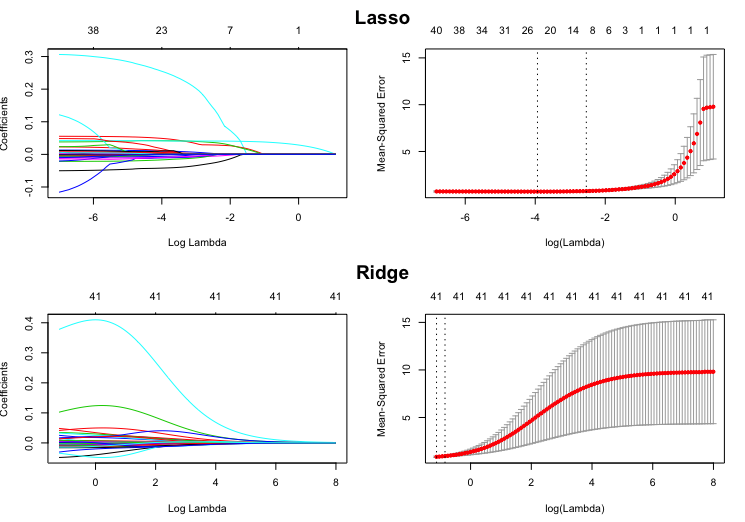
\includegraphics[scale = 1.3]{images/Regression.png}
         \caption{\color {black} Regression Results - Tobins Q with the SXXP dataset}
         \end{figure}
         {\large \color{black} Clearly, as $\lambda$ increase the model simplifies, however this is associated with an increase in MSE. This exemplifies the tradeoff between model interpretability and performance involved here.    } \\
         {{\bf \large  \color{black} Causal Inference}} \\
         {\large \color{black} Below is an example result from the causal stage of this study. }\\~\\
         \setlength{\tabcolsep}{0.6em}
         {\renewcommand{\arraystretch}{1}%
         \begin{tabular}{ll}
	{\large \color{black}  Dataset} & {\large \color{black} S\&P 500 } \\
	{\large \color{black} Dependent Variable} & {\large \color{black} Tobins Q Score } \\
	{\large \color{black} Treatment} & {\color{black} CEO Comp $>$ median(CEO Comp)? 1 : 0}  \\
	{\large \color{black} Estimate ($\% \Delta $)} & {\large \color{black} (-0.06 $\sim$ -0.11)} \\~\\
	\end{tabular}  }
	 {\large \color{black} This can be interpreted as; CEO compensation above the median causes a decrease in Tobins Q by between 6\% and 11\%. Below, two (of many) sample matching plots are shown.  }\\~\\

	
	\begin{figure}[h!]
	\centering
	\footnotesize{\subfloat[\footnotesize{Asset}]{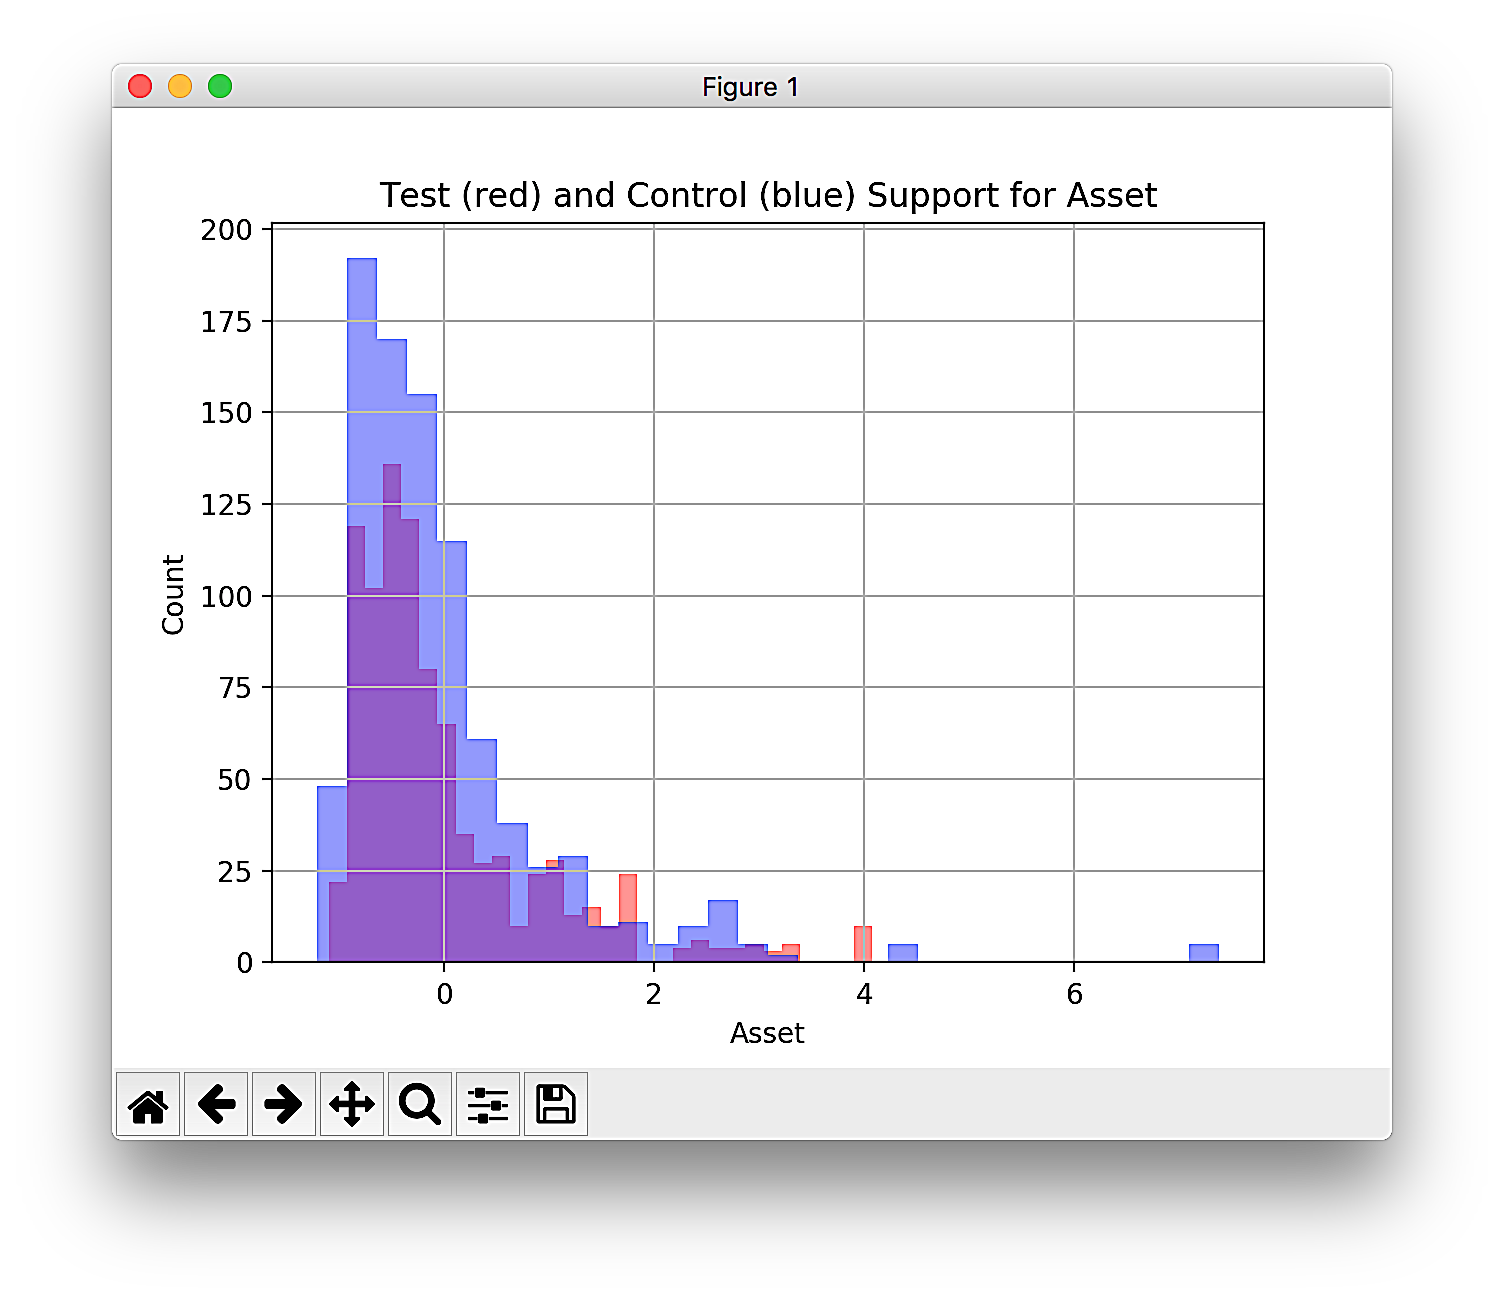
\includegraphics[width = 6in]{images/causal/CEOPayOverMedian/tobin/Asset.png}}}
	\footnotesize{\subfloat[\footnotesize{EBITDA 12Mth}]{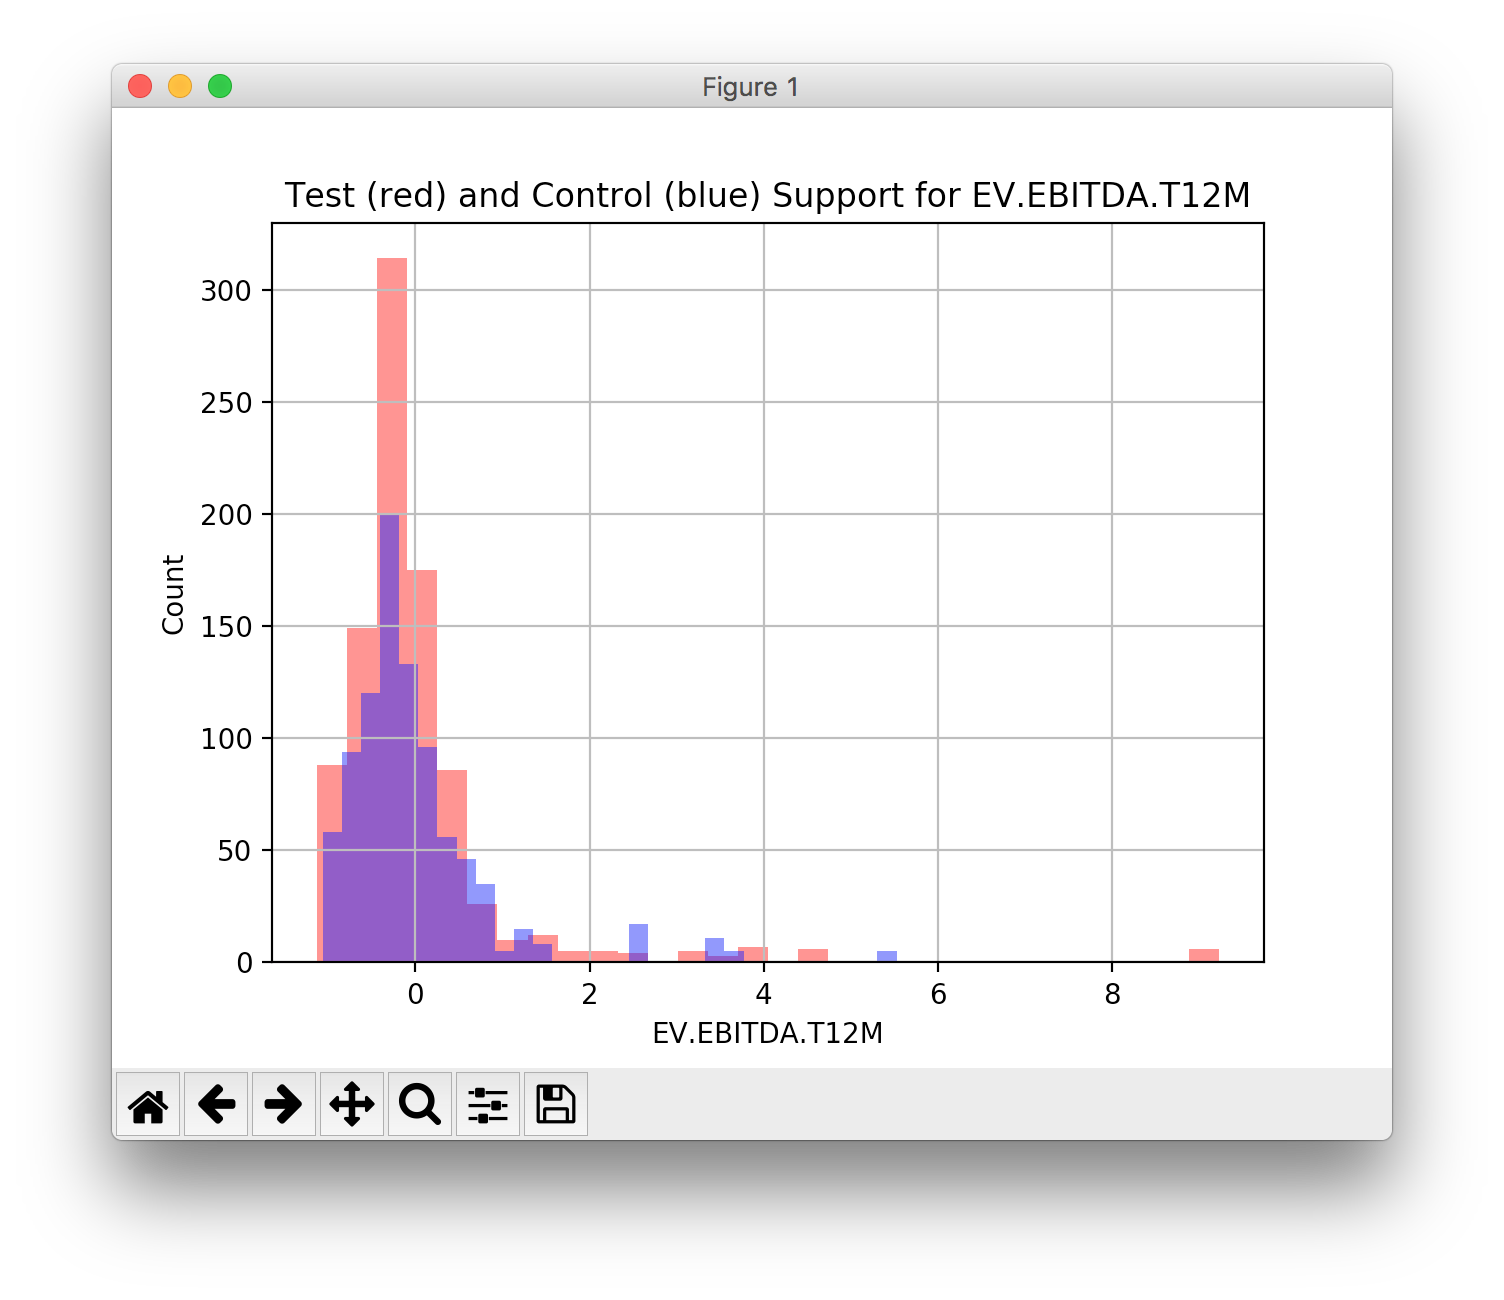
\includegraphics[width = 6in]{images/causal/CEOPayOverMedian/tobin/EV_EBITDA_T12M.png}} }
	\end{figure}
	\end{block}
	 \begin{block}{Conclusions}
          {\large \color{black} Previously identified {\it if-this-then-that} style rules for corporate governance best practice have been verified, by both replicating that previous study as well as reframing it in a more natural way as a regression problem. By utilising cutting edge causal techniques, a subset with causal merit were identified. The results of this study contribute to a growing literature base on corporate governance and its effects on economic outcomes.    }
	\end{block}
\end{column}

\begin{column}{\sepmargin} \end{column}
\end{columns} 

%\vspace{5cm}
	\begin{columns}[t] % Split up the two columns wide column again
	\begin{column}{\sepmargin} \end{column}
	\begin{column}{\onecolwid} % The first column
	\vspace*{-0.9cm}
	\begin{alertblock}{\large Contact Information}
	\vspace*{-0.5cm}
	\begin{footnotesize}
		\begin{itemize}
			\item {Conor Reid - MSc Business Analytics (Part Time)}
			\item \href{mailto:conor.reid@ucdconnect.ie}{conor.reid@ucdconnect.ie}
		\end{itemize}
	\end{footnotesize}	
	\end{alertblock}
	\end{column} % End of the first column
	\begin{column}{\sepwid}\end{column} % Empty spacer column
	\begin{column}{\onecolwid} % Begin a column 
	\begin{block}{\large References}
		\vspace*{-0.5cm}
              	\nocite{*} % Insert publications even if they are not cited in the poster
		{\footnotesize \bibliography{bibliog.bib}}
	\end{block} 
	\end{column} % End of the second column
%--------------------------------------------------------------------------------------------------------------------------------------------------------------------------------------------------------
\begin{column}{\sepmargin}\end{column} % Empty spacer column            
\end{columns} % End of all the columns in the poster
\end{frame} % End of the enclosing frame
\end{document}
